% Generated by Sphinx.
\def\sphinxdocclass{report}
\documentclass[letterpaper,10pt,french]{sphinxmanual}
\usepackage[utf8]{inputenc}
\DeclareUnicodeCharacter{00A0}{\nobreakspace}
\usepackage{cmap}
\usepackage[T1]{fontenc}
\usepackage{babel}
\usepackage{times}
\usepackage[Sonny]{fncychap}
\usepackage{longtable}
\usepackage{sphinx}
\usepackage{multirow}

\addto\captionsfrench{\renewcommand{\figurename}{Fig. }}
\addto\captionsfrench{\renewcommand{\tablename}{Tableau }}
\floatname{literal-block}{Code source }



\title{predictif Documentation}
\date{28 March 2015}
\release{0.1}
\author{H. Verlin - S. Toko}
\newcommand{\sphinxlogo}{}
\renewcommand{\releasename}{Version}
\makeindex

\makeatletter
\def\PYG@reset{\let\PYG@it=\relax \let\PYG@bf=\relax%
    \let\PYG@ul=\relax \let\PYG@tc=\relax%
    \let\PYG@bc=\relax \let\PYG@ff=\relax}
\def\PYG@tok#1{\csname PYG@tok@#1\endcsname}
\def\PYG@toks#1+{\ifx\relax#1\empty\else%
    \PYG@tok{#1}\expandafter\PYG@toks\fi}
\def\PYG@do#1{\PYG@bc{\PYG@tc{\PYG@ul{%
    \PYG@it{\PYG@bf{\PYG@ff{#1}}}}}}}
\def\PYG#1#2{\PYG@reset\PYG@toks#1+\relax+\PYG@do{#2}}

\expandafter\def\csname PYG@tok@s2\endcsname{\def\PYG@tc##1{\textcolor[rgb]{0.25,0.44,0.63}{##1}}}
\expandafter\def\csname PYG@tok@mi\endcsname{\def\PYG@tc##1{\textcolor[rgb]{0.13,0.50,0.31}{##1}}}
\expandafter\def\csname PYG@tok@k\endcsname{\let\PYG@bf=\textbf\def\PYG@tc##1{\textcolor[rgb]{0.00,0.44,0.13}{##1}}}
\expandafter\def\csname PYG@tok@mb\endcsname{\def\PYG@tc##1{\textcolor[rgb]{0.13,0.50,0.31}{##1}}}
\expandafter\def\csname PYG@tok@na\endcsname{\def\PYG@tc##1{\textcolor[rgb]{0.25,0.44,0.63}{##1}}}
\expandafter\def\csname PYG@tok@gh\endcsname{\let\PYG@bf=\textbf\def\PYG@tc##1{\textcolor[rgb]{0.00,0.00,0.50}{##1}}}
\expandafter\def\csname PYG@tok@kr\endcsname{\let\PYG@bf=\textbf\def\PYG@tc##1{\textcolor[rgb]{0.00,0.44,0.13}{##1}}}
\expandafter\def\csname PYG@tok@kp\endcsname{\def\PYG@tc##1{\textcolor[rgb]{0.00,0.44,0.13}{##1}}}
\expandafter\def\csname PYG@tok@w\endcsname{\def\PYG@tc##1{\textcolor[rgb]{0.73,0.73,0.73}{##1}}}
\expandafter\def\csname PYG@tok@cs\endcsname{\def\PYG@tc##1{\textcolor[rgb]{0.25,0.50,0.56}{##1}}\def\PYG@bc##1{\setlength{\fboxsep}{0pt}\colorbox[rgb]{1.00,0.94,0.94}{\strut ##1}}}
\expandafter\def\csname PYG@tok@nl\endcsname{\let\PYG@bf=\textbf\def\PYG@tc##1{\textcolor[rgb]{0.00,0.13,0.44}{##1}}}
\expandafter\def\csname PYG@tok@sr\endcsname{\def\PYG@tc##1{\textcolor[rgb]{0.14,0.33,0.53}{##1}}}
\expandafter\def\csname PYG@tok@gs\endcsname{\let\PYG@bf=\textbf}
\expandafter\def\csname PYG@tok@gu\endcsname{\let\PYG@bf=\textbf\def\PYG@tc##1{\textcolor[rgb]{0.50,0.00,0.50}{##1}}}
\expandafter\def\csname PYG@tok@nb\endcsname{\def\PYG@tc##1{\textcolor[rgb]{0.00,0.44,0.13}{##1}}}
\expandafter\def\csname PYG@tok@c1\endcsname{\let\PYG@it=\textit\def\PYG@tc##1{\textcolor[rgb]{0.25,0.50,0.56}{##1}}}
\expandafter\def\csname PYG@tok@mf\endcsname{\def\PYG@tc##1{\textcolor[rgb]{0.13,0.50,0.31}{##1}}}
\expandafter\def\csname PYG@tok@ni\endcsname{\let\PYG@bf=\textbf\def\PYG@tc##1{\textcolor[rgb]{0.84,0.33,0.22}{##1}}}
\expandafter\def\csname PYG@tok@sh\endcsname{\def\PYG@tc##1{\textcolor[rgb]{0.25,0.44,0.63}{##1}}}
\expandafter\def\csname PYG@tok@si\endcsname{\let\PYG@it=\textit\def\PYG@tc##1{\textcolor[rgb]{0.44,0.63,0.82}{##1}}}
\expandafter\def\csname PYG@tok@kd\endcsname{\let\PYG@bf=\textbf\def\PYG@tc##1{\textcolor[rgb]{0.00,0.44,0.13}{##1}}}
\expandafter\def\csname PYG@tok@mo\endcsname{\def\PYG@tc##1{\textcolor[rgb]{0.13,0.50,0.31}{##1}}}
\expandafter\def\csname PYG@tok@no\endcsname{\def\PYG@tc##1{\textcolor[rgb]{0.38,0.68,0.84}{##1}}}
\expandafter\def\csname PYG@tok@il\endcsname{\def\PYG@tc##1{\textcolor[rgb]{0.13,0.50,0.31}{##1}}}
\expandafter\def\csname PYG@tok@gt\endcsname{\def\PYG@tc##1{\textcolor[rgb]{0.00,0.27,0.87}{##1}}}
\expandafter\def\csname PYG@tok@o\endcsname{\def\PYG@tc##1{\textcolor[rgb]{0.40,0.40,0.40}{##1}}}
\expandafter\def\csname PYG@tok@cm\endcsname{\let\PYG@it=\textit\def\PYG@tc##1{\textcolor[rgb]{0.25,0.50,0.56}{##1}}}
\expandafter\def\csname PYG@tok@sb\endcsname{\def\PYG@tc##1{\textcolor[rgb]{0.25,0.44,0.63}{##1}}}
\expandafter\def\csname PYG@tok@gi\endcsname{\def\PYG@tc##1{\textcolor[rgb]{0.00,0.63,0.00}{##1}}}
\expandafter\def\csname PYG@tok@vi\endcsname{\def\PYG@tc##1{\textcolor[rgb]{0.73,0.38,0.84}{##1}}}
\expandafter\def\csname PYG@tok@c\endcsname{\let\PYG@it=\textit\def\PYG@tc##1{\textcolor[rgb]{0.25,0.50,0.56}{##1}}}
\expandafter\def\csname PYG@tok@go\endcsname{\def\PYG@tc##1{\textcolor[rgb]{0.20,0.20,0.20}{##1}}}
\expandafter\def\csname PYG@tok@s1\endcsname{\def\PYG@tc##1{\textcolor[rgb]{0.25,0.44,0.63}{##1}}}
\expandafter\def\csname PYG@tok@nf\endcsname{\def\PYG@tc##1{\textcolor[rgb]{0.02,0.16,0.49}{##1}}}
\expandafter\def\csname PYG@tok@m\endcsname{\def\PYG@tc##1{\textcolor[rgb]{0.13,0.50,0.31}{##1}}}
\expandafter\def\csname PYG@tok@bp\endcsname{\def\PYG@tc##1{\textcolor[rgb]{0.00,0.44,0.13}{##1}}}
\expandafter\def\csname PYG@tok@nc\endcsname{\let\PYG@bf=\textbf\def\PYG@tc##1{\textcolor[rgb]{0.05,0.52,0.71}{##1}}}
\expandafter\def\csname PYG@tok@vc\endcsname{\def\PYG@tc##1{\textcolor[rgb]{0.73,0.38,0.84}{##1}}}
\expandafter\def\csname PYG@tok@sx\endcsname{\def\PYG@tc##1{\textcolor[rgb]{0.78,0.36,0.04}{##1}}}
\expandafter\def\csname PYG@tok@ne\endcsname{\def\PYG@tc##1{\textcolor[rgb]{0.00,0.44,0.13}{##1}}}
\expandafter\def\csname PYG@tok@gp\endcsname{\let\PYG@bf=\textbf\def\PYG@tc##1{\textcolor[rgb]{0.78,0.36,0.04}{##1}}}
\expandafter\def\csname PYG@tok@nv\endcsname{\def\PYG@tc##1{\textcolor[rgb]{0.73,0.38,0.84}{##1}}}
\expandafter\def\csname PYG@tok@kc\endcsname{\let\PYG@bf=\textbf\def\PYG@tc##1{\textcolor[rgb]{0.00,0.44,0.13}{##1}}}
\expandafter\def\csname PYG@tok@ge\endcsname{\let\PYG@it=\textit}
\expandafter\def\csname PYG@tok@nt\endcsname{\let\PYG@bf=\textbf\def\PYG@tc##1{\textcolor[rgb]{0.02,0.16,0.45}{##1}}}
\expandafter\def\csname PYG@tok@kn\endcsname{\let\PYG@bf=\textbf\def\PYG@tc##1{\textcolor[rgb]{0.00,0.44,0.13}{##1}}}
\expandafter\def\csname PYG@tok@nd\endcsname{\let\PYG@bf=\textbf\def\PYG@tc##1{\textcolor[rgb]{0.33,0.33,0.33}{##1}}}
\expandafter\def\csname PYG@tok@kt\endcsname{\def\PYG@tc##1{\textcolor[rgb]{0.56,0.13,0.00}{##1}}}
\expandafter\def\csname PYG@tok@nn\endcsname{\let\PYG@bf=\textbf\def\PYG@tc##1{\textcolor[rgb]{0.05,0.52,0.71}{##1}}}
\expandafter\def\csname PYG@tok@ss\endcsname{\def\PYG@tc##1{\textcolor[rgb]{0.32,0.47,0.09}{##1}}}
\expandafter\def\csname PYG@tok@gr\endcsname{\def\PYG@tc##1{\textcolor[rgb]{1.00,0.00,0.00}{##1}}}
\expandafter\def\csname PYG@tok@sd\endcsname{\let\PYG@it=\textit\def\PYG@tc##1{\textcolor[rgb]{0.25,0.44,0.63}{##1}}}
\expandafter\def\csname PYG@tok@se\endcsname{\let\PYG@bf=\textbf\def\PYG@tc##1{\textcolor[rgb]{0.25,0.44,0.63}{##1}}}
\expandafter\def\csname PYG@tok@gd\endcsname{\def\PYG@tc##1{\textcolor[rgb]{0.63,0.00,0.00}{##1}}}
\expandafter\def\csname PYG@tok@sc\endcsname{\def\PYG@tc##1{\textcolor[rgb]{0.25,0.44,0.63}{##1}}}
\expandafter\def\csname PYG@tok@ow\endcsname{\let\PYG@bf=\textbf\def\PYG@tc##1{\textcolor[rgb]{0.00,0.44,0.13}{##1}}}
\expandafter\def\csname PYG@tok@err\endcsname{\def\PYG@bc##1{\setlength{\fboxsep}{0pt}\fcolorbox[rgb]{1.00,0.00,0.00}{1,1,1}{\strut ##1}}}
\expandafter\def\csname PYG@tok@mh\endcsname{\def\PYG@tc##1{\textcolor[rgb]{0.13,0.50,0.31}{##1}}}
\expandafter\def\csname PYG@tok@vg\endcsname{\def\PYG@tc##1{\textcolor[rgb]{0.73,0.38,0.84}{##1}}}
\expandafter\def\csname PYG@tok@cp\endcsname{\def\PYG@tc##1{\textcolor[rgb]{0.00,0.44,0.13}{##1}}}
\expandafter\def\csname PYG@tok@s\endcsname{\def\PYG@tc##1{\textcolor[rgb]{0.25,0.44,0.63}{##1}}}

\def\PYGZbs{\char`\\}
\def\PYGZus{\char`\_}
\def\PYGZob{\char`\{}
\def\PYGZcb{\char`\}}
\def\PYGZca{\char`\^}
\def\PYGZam{\char`\&}
\def\PYGZlt{\char`\<}
\def\PYGZgt{\char`\>}
\def\PYGZsh{\char`\#}
\def\PYGZpc{\char`\%}
\def\PYGZdl{\char`\$}
\def\PYGZhy{\char`\-}
\def\PYGZsq{\char`\'}
\def\PYGZdq{\char`\"}
\def\PYGZti{\char`\~}
% for compatibility with earlier versions
\def\PYGZat{@}
\def\PYGZlb{[}
\def\PYGZrb{]}
\makeatother

\renewcommand\PYGZsq{\textquotesingle}

\begin{document}

\maketitle
\tableofcontents
\phantomsection\label{index::doc}



\chapter{Table des matières}
\label{index:prefictif-documentation}\label{index:table-des-matieres}

\section{Modèle du domaine}
\label{modele:modele-du-domaine}\label{modele::doc}

\subsection{Liste des entity}
\label{modele:liste-des-entity}
L'analyse des besoins concernant cette application nous a permis de définir ces différentes classes :

\begin{tabulary}{\linewidth}{|L|L|}
\hline
\textsf{\relax 
Nom
} & \textsf{\relax 
Fonction
}\\
\hline
Client
 & 
Client de predict'if
\\
\hline
Employe
 & 
Employe de Predict'if
\\
\hline
Medium
 & 
Medium fictif
\\
\hline
Horoscope
 & 
Horoscope contenant un ensemble de 3 prédictions de type différent
\\
\hline
Prédiction
 & 
Classe abstraite qui sert de base pour les 3 types de prédictions
\\
\hline
PrédictionAmour
 & 
Prédiction de catégorie Amour,
indique un signe partenaire
\\
\hline
PrédictionTravail
 & 
Prédiction de catégorie Travail
\\
\hline
PrédictionSante
 & 
Prediction de catégorie Santé, contient un conseil pour le client
\\
\hline
Signe
 & 
Réprésente un signe astrologique simplifié
(correspond à un mois de l'année)
\\
\hline\end{tabulary}



\subsection{Diagramme de Classes}
\label{modele:diagramme-de-classes}
Le diagramme de classes ci-dessous reprend les différentes classes présentés ci-dessus.

{\hfill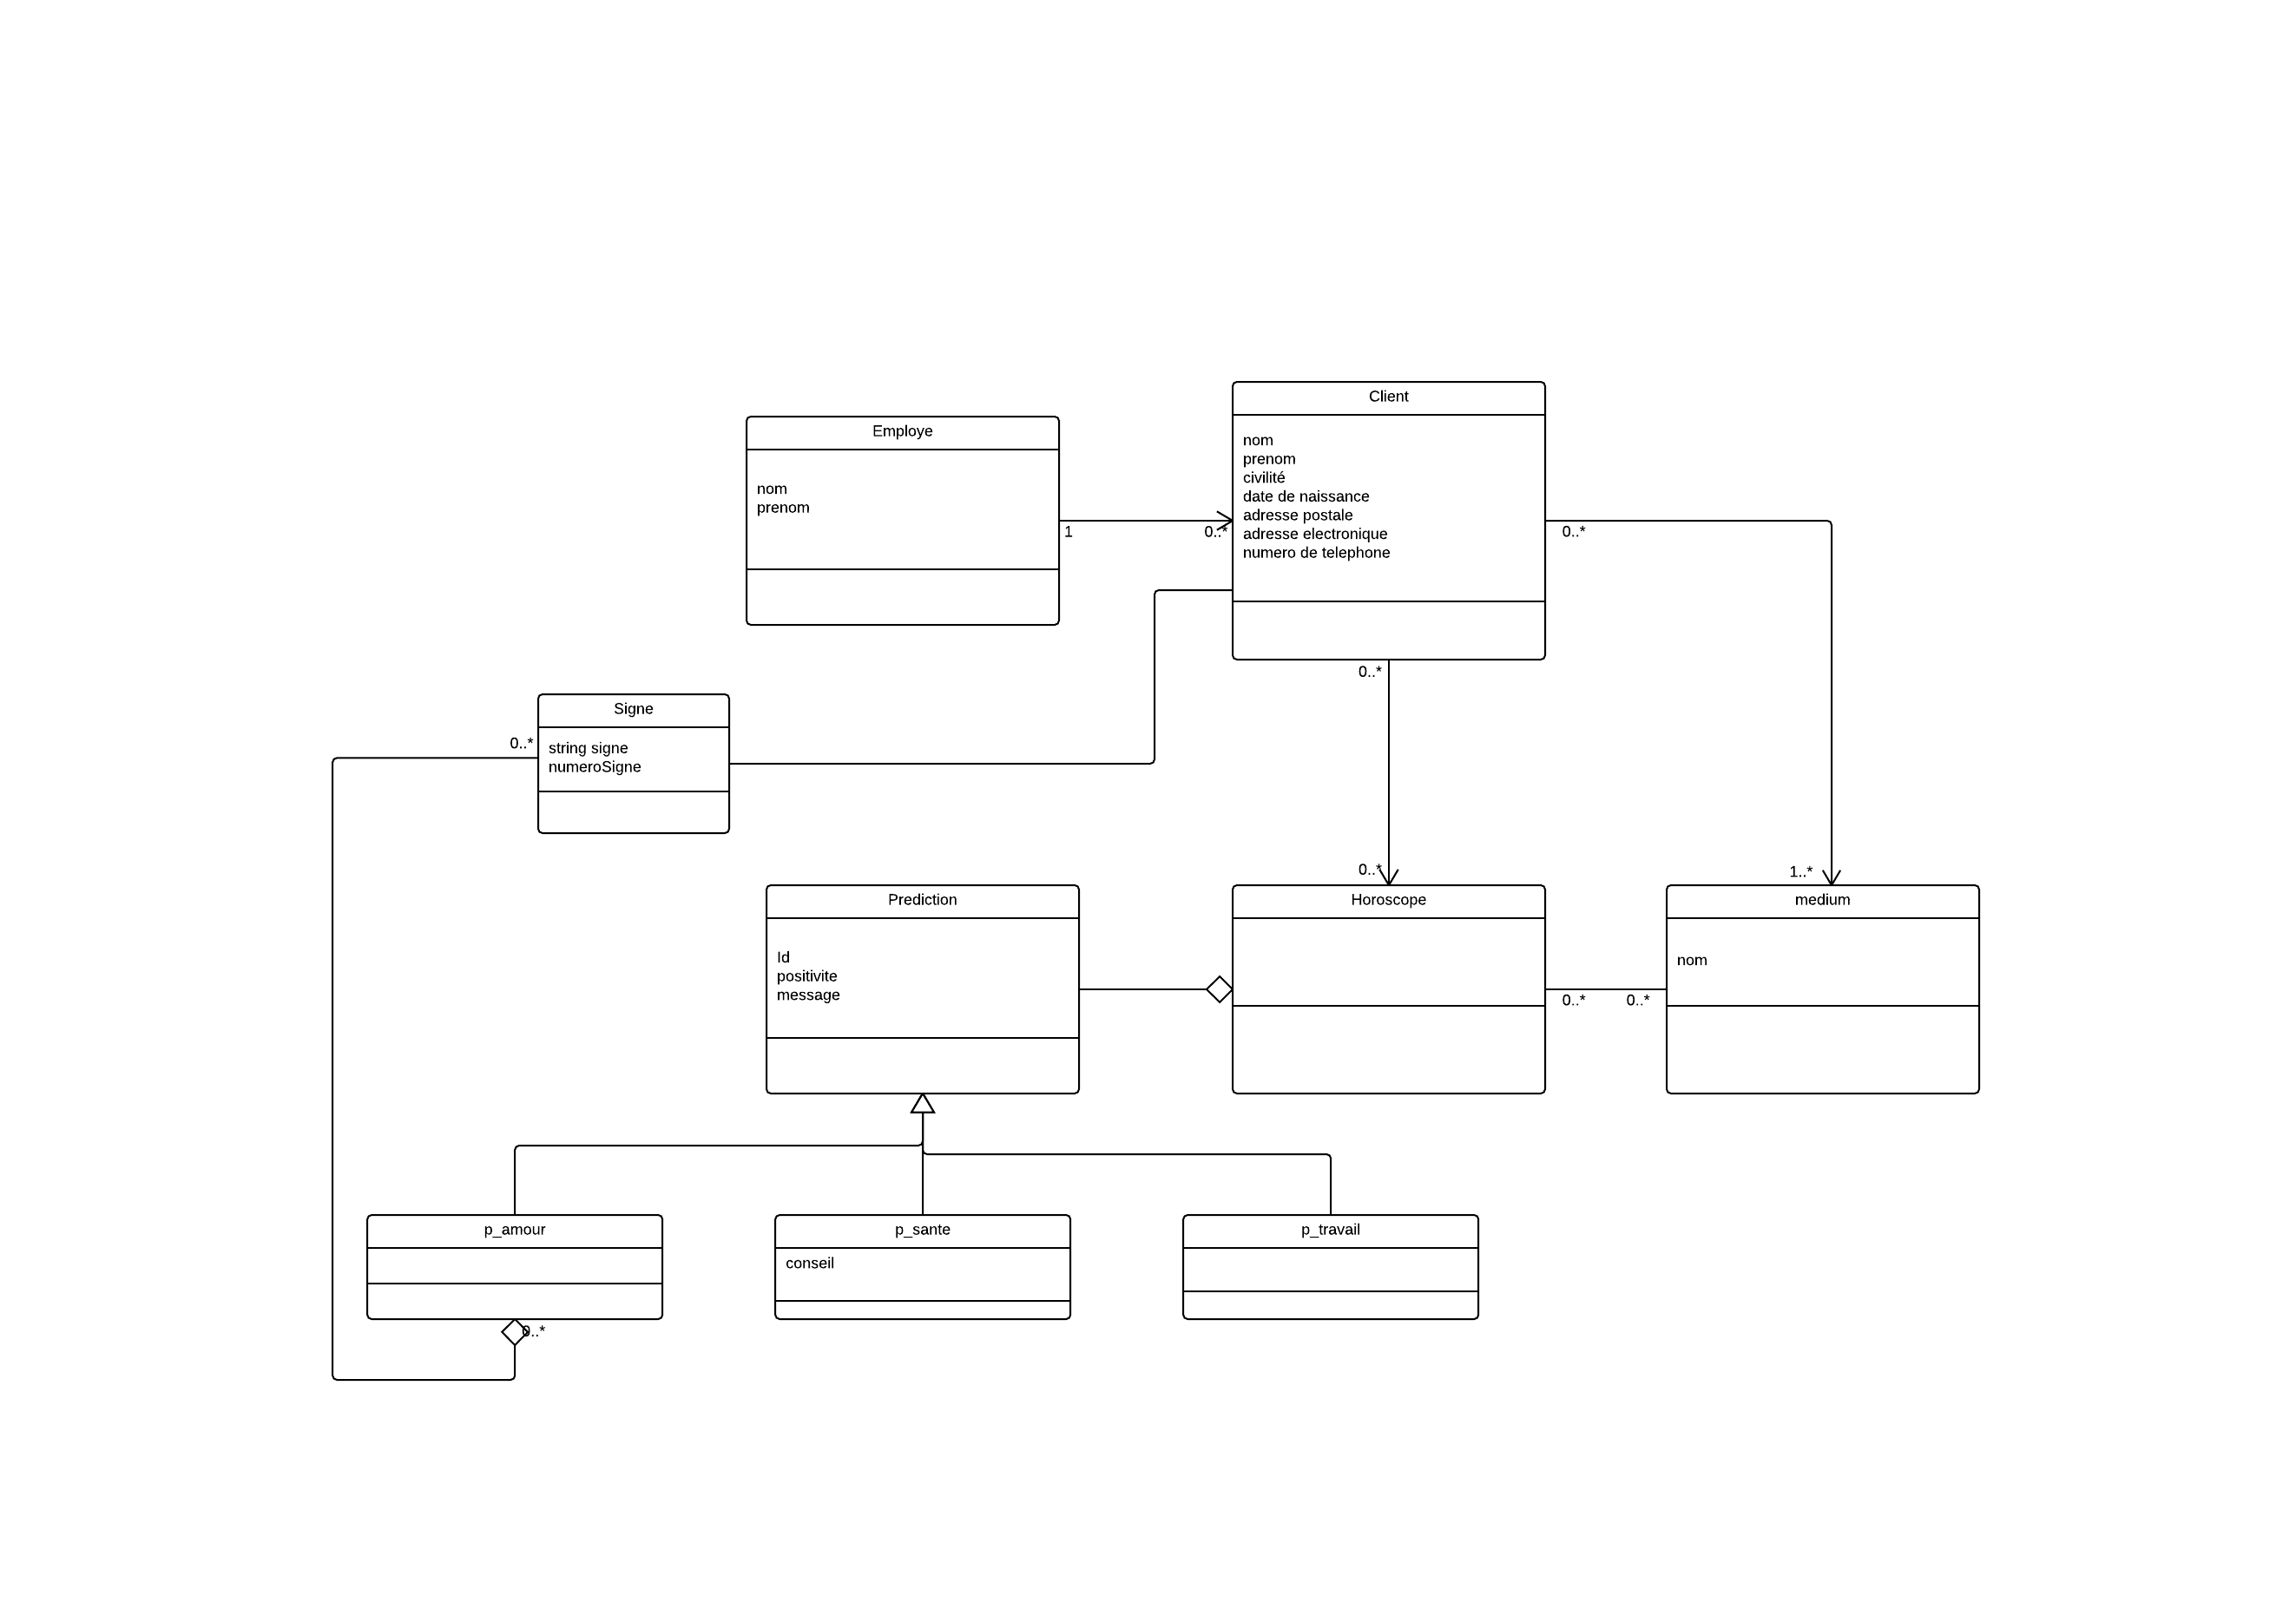
\includegraphics{uml.png}\hfill}


\section{Présentation des maquettes}
\label{maquette:presentation-des-maquettes}\label{maquette::doc}

\section{Description des services}
\label{services::doc}\label{services:description-des-services}
\begin{tabulary}{\linewidth}{|L|L|L|}
\hline
\textsf{\relax 
Méthode
} & \textsf{\relax 
Retour
} & \textsf{\relax 
Brève Description
}\\
\hline
creerClient(Client client)
 & 
int
 & 
Permet d'insérer un client dans la base de données
\\
\hline
creerEmploye(Employe employe)
 & 
void
 & 
Permet d'insérer un employé dans la base de données
\\
\hline
creerHoroscope(Horoscope horoscope, Client client)
 & 
void
 & 
Permet d'insérer un horoscope dans la base de données,
et de l'attacher à un client.
Elle simule l'envoi du mail au client
\\
\hline
creerMedium(Medium medium)
 & 
void
 & 
Permet d'insérer un signe dans la base de données
\\
\hline
creerPredictionAmour(PredictionAmour predictionAmour)
 & 
void
 & 
Permet d'insérer une prédiction de type amour dans la base de données
\\
\hline
creerPredictionSante(PredictionSante predictionSante)
 & 
void
 & 
Permet d'insérer une prédiction de type santé dans la base de données
\\
\hline
creerPredictionTravail(PredictionTravail predictionTravail)
 & 
void
 & 
Permet d'insérer une prédiction de type travail dans la base de données
\\
\hline
creerSigne(Signe signe)
 &  & 
Permet d'insérer un signe dans la base de données
\\
\hline
getClientById(long idClient)
 & 
Client
 & 
Récupère un client grâce à son id
\\
\hline
listerClients()
 & 
List\textless{}Client\textgreater{}
 & 
Liste de toutes les clients de la base
\\
\hline
listerHistoriqueClient(Client client)
 & 
List\textless{}Horoscope\textgreater{}
 & 
Renvoie l'historique de l'horoscope d'un client
\\
\hline
listerMediums()
 & 
List\textless{}Medium\textgreater{}
 & 
Liste de tous les mediums de la base
\\
\hline
listerMediumsClient(Client client)
 & 
List\textless{}Medium\textgreater{}
 & 
Liste tous les mediums d'un client
\\
\hline
listerPredictionAmours()
 & 
List\textless{}PredictionAmour\textgreater{}
 & 
Liste de toutes les predictions amour de la base
\\
\hline
listerPredictionSantes()
 & 
List\textless{}PredictionSante\textgreater{}
 & 
Liste de toutes les predictions sante de la base
\\
\hline
listerPredictionTravails()
 & 
List\textless{}PredictionTravail\textgreater{}
 & 
Liste de toutes les predictions travail de la base
\\
\hline
listerSignes()
 & 
List\textless{}Signe\textgreater{}
 & 
Liste de toutes les signes de la base
\\
\hline
updateEmp(Employe emp)
 & 
void
 & 
Met à jour un employé dans la base
\\
\hline\end{tabulary}



\chapter{Introduction}
\label{index:introduction}
\emph{Prédict’IF} est un cabinet de voyance en ligne, qui envoie périodiquement des email à ses clients. Ces emails contiennent des horoscopes personnalisés créés par les employés de l'entreprise. Ceux-ci se basent sur le signe du client, et sur le choix des voyants qu'il a séléctionné lors de son inscription.

Les services présentés ici permettent a création des différentes briques de l'application Prédict’IF, c'est-à-dire à la réalisation des différentes IHM.

L'ensemble des services fournis permet la réalisation de deux IHM :
\begin{itemize}
\item {} 
Une IHM web pour les clients, qui leur permet de s'inscrire pour recevoir des horoscopes

\item {} 
Une IHM web pour les employés, pour la réalisation des horoscopes

\end{itemize}

Vous trouverez dans cette documentation :
\begin{enumerate}
\item {} 
Le modèle du domain avec un diagramme de classe UML

\item {} 
La maquette des 3 IHM (président, employés, clients)

\item {} 
La description des services

\end{enumerate}



\renewcommand{\indexname}{Index}
\printindex
\end{document}
